%%%%%%%%%%%%%%%%%%%%%%%%%%%%%%%%%%%%%%%%%
%
% (c) 2018 by Jennifer Laaser
%
% This work is licensed under the Creative Commons Attribution-NonCommercial-ShareAlike 4.0 International License. To view a copy of this license, visit http://creativecommons.org/licenses/by-nc-sa/4.0/ or send a letter to Creative Commons, PO Box 1866, Mountain View, CA 94042, USA.
%
% The current source for these materials is accessible on Github: https://github.com/jlaaser/pogil-polymers
%
%%%%%%%%%%%%%%%%%%%%%%%%%%%%%%%%%%%%%%%%%

\renewcommand{\figpath}{content/polymchem/stepgrowth/condensation-equilibria/figs}
\renewcommand{\labelbase}{condequilib}

\begin{activity}{Equilibrium in Condensation Polymerizations}

\begin{instructornotes}

	This activity introduces students to the role of chemical equilibria in condensation polymerizations.
	
	After completing this activity, students will be able to:
			\begin{enumerate}
				\item Explain how chemical equilibrium affects the extent of reaction in condensation polymerizations
				\item Explain how reaction conditions can be manipulated to produce high molecular-weight polymers
				\item Apply these concepts to the analysis of commercially-important polymer syntheses
			\end{enumerate}
	
			
	\subsection*{Activity summary:}
	\begin{itemize}
		\item \textbf{Activity type:} Learning Cycle
		\item \textbf{Content goals:} Equilibrium effects in condensation polymerizations
		\item \textbf{Process goals:} %https://pogil.org/uploads/attachments/cj54b5yts006cklx4hh758htf-process-skills-official-pogil-list-2015-original.pdf
			written communication, critical thinking, information processing
		\item \textbf{Duration:} approx. 45 minutes
		\item \textbf{Instructor preparation required:} none beyond knowledge of relevant content
		\item \textbf{Related textbook chapters:}
			\begin{itemize}
				\item \emph{Polymer Chemistry} (Hiemenz \& Lodge): Not covered in detail, but some information in sections 2.5 and 2.6
			\end{itemize}
	\end{itemize}

\end{instructornotes}

	%\textbf{Focus question:} Put a central question for the students to consider through this exercise here.

\begin{model}[Equilibria in Condensation Reactions]

	So far, we have written all reactions as unidirectional, proceeding only from \emph{reactants} to \emph{products}.
	However, in reality, the reactions used to produce polymers by step-growth polymerization are typically reversible, and proceed under equilibrium conditions.
	
	This issue is particularly important for condensation reactions, which produce a small-molecule byproduct.
	Consider the reaction of an ``A'' functional group with a ``B'' functional group to produce an ``ab'' bond:
	
		\vspace{0.1in}
		\centerline{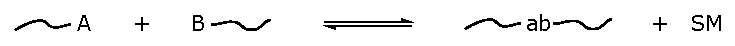
\includegraphics[width=0.9\textwidth]{\figpath/model1-rxnscheme.pdf}}
	
	Here, we have included the small molecule byproduct, ``SM'' on the right side of the reaction.
	We have also written the reaction arrow as a double arrow ($\rightleftharpoons$) to indicate that the reaction is reversible.

\end{model}


\begin{ctqs}

	\question \label{\labelbase:ctq:Keq} Write an expression for the equilibrium constant for this reaction, $K_{eq}$, in terms of the concentrations of A groups ([A]), B groups ([B]), ab bonds ([ab]), and released small molecules ([SM]):
	
		\begin{solution}[1in]
			\begin{equation*}
				K_{eq} = \frac{[ab][SM]}{[A][B]}
			\end{equation*}
		\end{solution}
	
	\question \label{\labelbase:ctq:ICE} Suppose we start with $v_A^0$ A groups.  If the reaction is stoichiometrically balanced, that means we also start with $v_A^0$ B groups.
	
		Using this information, complete the following ICE table:
		\begin{center}
			\renewcommand{\arraystretch}{4}
			\begin{tabular}{|c|c|c|c|c|}
				\hline
				~ & ~~~~~~~\textbf{A}~~~~~~~ & ~~~~~~~\textbf{B}~~~~~~~ & ~~~~~~~\textbf{ab}~~~~~~~ & ~~~~~~~\textbf{SM}~~~~~~~\\\hline
				\textbf{Initial} & $v_A^0$ & $v_A^0$ & 0 & 0 \\\hline
				\textbf{Change} & $-x$ & \answer{$-x$} & \answer{$+x$} & \answer{$+x$} \\\hline
				\textbf{Equilibrium} & \answer{$v_A^0 - x$} & $v_A^0-x$ & \answer{$x$} & \answer{$x$} \\\hline
			\end{tabular}
		\end{center}
		
	\question Plug your values from the equilibrium line of this table into your expression from CTQ \ref{\labelbase:ctq:Keq} to find an expression for $K_{eq}$ in terms of $v_A^0$ and $x$.
	
		\emph{Note: your expression from CTQ \ref{\labelbase:ctq:Keq} is written in terms of concentrations, while the values in the table in CTQ \ref{\labelbase:ctq:ICE} are written in terms of numbers of molecules.  In this problem, however, it turns out that things cancel such that you can just directly plug the values from CTQ \ref{\labelbase:ctq:ICE} into the expression from CTQ \ref{\labelbase:ctq:Keq} directly.}
	
		\begin{solution}[1.05in]
			\begin{equation*}
				K_{eq} = \frac{x^2}{(v_A^0-x)^2}
			\end{equation*}
		\end{solution}
	
	\question  When the extent of reaction is equal to $p$, the number of $A$ groups that have reacted is $pv_A^0$, so $x=pv_A^0$.   Using this information, rewrite $K_{eq}$ only in terms of $p$.
	
		\emph{Hint: to make the next question easier, leave the denominator in the form $(1-p)^2$ instead of multiplying it out.}
		
		\begin{solution}[1.25in]
			\begin{equation*}
				K_{eq} = \frac{(pV_A^0)^2}{(v_A^0 - pv_A^0)^2} = \frac{p^2}{(1-p)^2}
			\end{equation*}
		\end{solution}
		
	\question Solve for $p$ in terms of $K_{eq}$.
	\label{\labelbase:ctq:Keqp}
		
		\emph{Hint: start by taking the square root of both sides of the equation.}
	
		\begin{solution}[3.25in]
			\begin{equation*}
				\sqrt{K_{eq}} = \sqrt{\frac{p^2}{(1-p)^2}} = \frac{p}{1-p}
			\end{equation*}
			so
			\begin{align*}
				(1-p)\sqrt{K_{eq}} &= p\\
				\sqrt{K_{eq}} &= p + p\sqrt{K_{eq}}  \\
				p &= \frac{\sqrt{K_{eq}}}{1+\sqrt{K_{eq}}}
			\end{align*}
		\end{solution}
	
	
	\question Finally, recalling that the number-average degree of polymerization is related to $p$ by $N_n = \frac{1}{1-p}$, find an expression for $N_n$ in terms of $K_{eq}$.
		
		\begin{solution}[4.5in]
			\begin{align*}
				N_n &= \frac{1}{1-p} \\
				&= \frac{1}{1-\frac{\sqrt{K_{eq}}}{1+\sqrt{K_{eq}}}}\\
				&= \frac{1+\sqrt{K_{eq}}}{1+\sqrt{K_{eq}} - \sqrt{K_{eq}}}\\
				&= 1+ \sqrt{K_{eq}}
			\end{align*}
		\end{solution}
		
\end{ctqs}
	
\clearpage % otherwise, this begins awkwardly at the end of one page
\begin{model}[Equilibrium in Condensation Polymerizations]
\label{\labelbase:mdl:K}

Polyesters and polyamides are two important classes of polymers formed by condensation polymerization.

Shown below are the bond-forming reactions and range of equilibrium constants for typical esterification and amidation reactions:
	
		\vspace{0.1in}
		\centerline{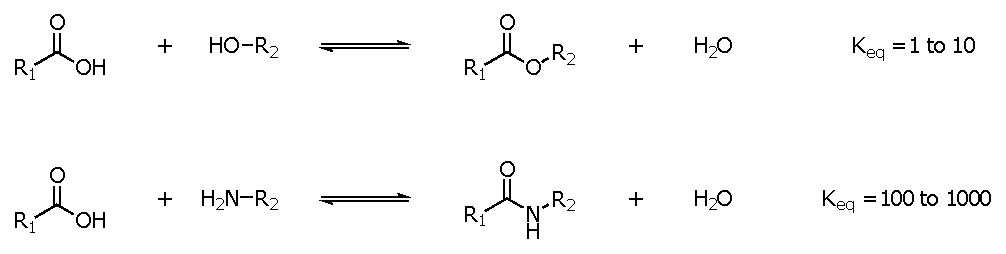
\includegraphics[width=0.9\textwidth]{\figpath/model2-esteramide.pdf}}

\end{model}

\begin{ctqs}
		\question Calculate the range of $N_n$ values you would expect for a polyester synthesized under equilibrium conditions.
		
			\begin{solution}[2in]
			
				When $K_{eq}=1$, $N_n = 1+ \sqrt{1} = 2$.
			
				When $K_{eq}=10$, $N_n = 1+ \sqrt{10} = 4.2$.
				
				Thus for a polyester synthesized under equilibrium conditions, we would expect to achieve a degree of polymerization of only about 2-4 (which is hardly a polymer!).			
			
			\end{solution}
		
		\question Calculate the range of $N_n$ values you would expect for a polyamide synthesized under equilibrium conditions.
		
			\begin{solution}[2in]
			
				When $K_{eq}=100$, $N_n = 1+ \sqrt{100} = 11$.
			
				When $K_{eq}=1000$, $N_n = 1+ \sqrt{1000} = 33$.
				
				Thus for a polyamide synthesized under equilibrium conditions, we would expect to achieve a degree of polymerization somewhere between 10 and 30.
			\end{solution}
		
\end{ctqs}

\begin{infobox}

	Commercial applications of polyesters and polyamides typically require degrees of polymerization of 100 or more.  

\end{infobox}

\begin{ctqs}
		
		\question Can commercial polyesters and polyamides be produced under equilibrium conditions?  Why or why not?
		
			\begin{solution}[2in]
			
				No. As seen above, synthesizing these polymers under equilibrium conditions results in degrees of polymerization of less than 50.  This is not long enough for commercial applications requiring degrees of polymerization of 100 or more.
			
			\end{solution}
			
		\question Propose at least one way that you could increase the degree of polymerization for polymers produced using the reactions shown in Model \ref{\labelbase:mdl:K}.  Explain your proposed solution in 2-3 complete sentences.
		
			\emph{Hint: you will probably want to think about this question in the context of Le Chatelier's principle.}
		
			\begin{solution}[2.5in]
			
				Le Chatelier's principle tells us that if a system in dynamic equilibrium is subjected to some stress, then the equilibrium will shift to relieve that stress.
				
				Practically speaking, that means that if we want to push the reaction toward the products (which will help us achieve a higher extent of reaction, and thus produce longer polymer chains), we should remove the small molecule byproduct as it is produced.
				
				The easiest way to do this will be to (1) run the reaction in an open system, and (2) run it at high temperature so that the small molecule byproduct (e.g. water) is vaporized and can escape.
			
			\end{solution}
		
\end{ctqs}

\clearpage
\begin{model}[Synthesis of Polyethylene Terephthalate]
\label{\labelbase:mdl:PET}

One commercially-important polyester produced by condensation polymerization is polyethylene terephthalate, or PET.
PET is produced in quantities of more than 9 billion pounds per year, and is used in drink bottles, plastic films, and many other products.

PET is produced in a two-step transesterification process, as shown below:
	
		\vspace{0.1in}
		\centerline{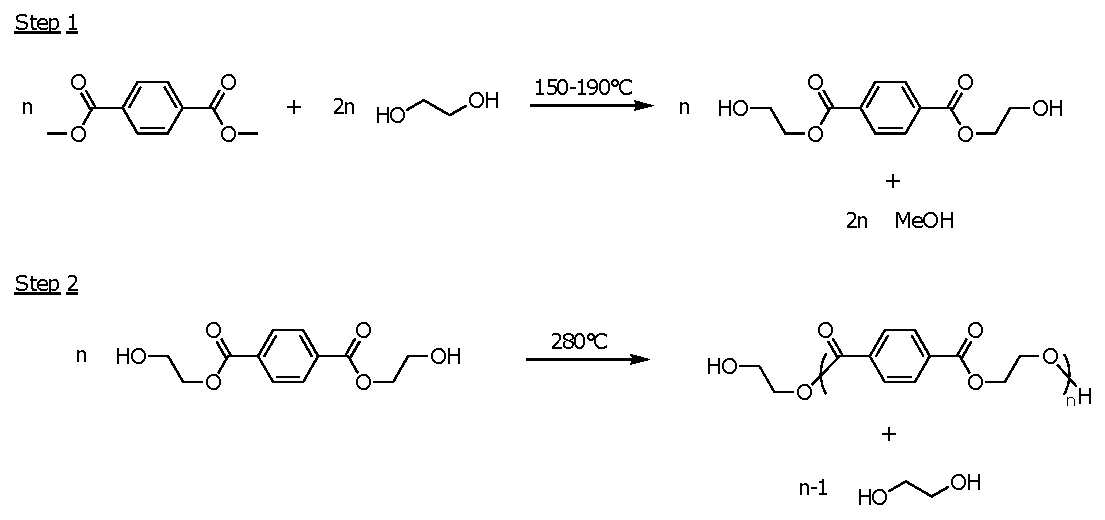
\includegraphics[width=\textwidth]{\figpath/model3-PETsynthesis.pdf}}

\end{model}

\begin{ctqs}
		

			
		\question What small molecule is released in the transesterification reaction shown in Step 1?
		
			\begin{solution}[0.75in]
				Methanol (\ce{CH3OH})
			\end{solution}
		
		\question What small molecule is released in the transesterification reaction shown in Step 2?
		
			\begin{solution}[0.75in]
				\instructordisplay{Ethylene glycol (\ce{HOCH2CH2OH}):
				
				\centerline{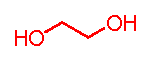
\includegraphics[width=0.15\textwidth]{\figpath/model3-glycol-red.pdf}}
				}
			\end{solution}
			
\end{ctqs}

\begin{infobox}
	
	The boiling point of methanol is 64.7${}^\circ$C.
	
	The boiling point of ethylene glycol (\ce{HOCH2CH2OH}) is 196${}^\circ$C.
	
\end{infobox}

\begin{ctqs}
	
	\question Why is the reaction in Step 1 carried out between 150 and 190${}^\circ$C?  Briefly explain your answer in 1-2 complete sentences.
	
		\begin{solution}[2in]
			The reaction in Step 1 is carried out between 150 and 190${}^\circ$C so that the methanol produced in the reaction will boil off/exit the system and help push the reaction toward the oligomer product.
		\end{solution}
	
	\question Why is the reaction in Step 2 carried out at 280${}^\circ$C?  Briefly explain your answer in 1-2 complete sentences.
	
		\begin{solution}[2in]
			The reaction in Step 2 is carried out at 280${}^\circ$C so that the ethylene glycol produced in the reaction will boil off/exit the system and help push the reaction toward the polymer product.
		\end{solution}
	
	\question If we attempted to run the reaction in Step 1 at 280${}^\circ$C, would we form the desired polymer? Why or why not?
	
		\begin{solution}[2in]
			We probably would not form the desired polymer product; this temperature is high enough that much of the ethylene glycol starting material would likely boil off before the reaction could progress significantly toward the desired product.
		\end{solution}
		
\end{ctqs}
	


\begin{exercises}

		\exercise Both of the reactions shown in Model \ref{\labelbase:mdl:K} produced water (\ce{H2O}) as the small-molecule byproduct.  However, if we had started with acid chloride reagents, we might instead produce \ce{HCl} as the small-molecule byproduct:
		
		\centerline{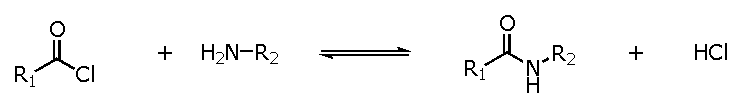
\includegraphics[width=0.8\textwidth]{\figpath/exercises-amidewithchloride.pdf}}
		
		Explain why, in this case, adding a stoichiometric amount of triethylamine should help promote formation of high molecular weight products.
		
			\begin{solution}
				\instructordisplay{
					Triethylamine will react with the \ce{HCl} product to form triethylammonium chloride.  This effectively removes the \ce{HCl} product from the reaction, helping pull the equilibrium toward the products.  This increases the overall extent of reaction and increases the molecular weight of the products.
				}
			\end{solution}
			
		\exercise Explain, in complete sentences, why the reactions shown in Model \ref{\labelbase:mdl:PET} are both referred to as ``trans-esterification'' reactions.
		
			\emph{Hint: what types of bonds are broken in each reaction, and what types of bonds are formed?  How does this differ from the other esterification reactions you have studied in this class?}
			
			\begin{solution}
				\instructordisplay{
				In both reactions, both the reagents and the products contain an ester bond and an alcohol (or hydroxyl).  When these reagents undergo transesterification, the initial ester is broken apart, and a new ester is formed with a different hydroxyl-bearing compound.
				
				By contrast, in the other esterification reactions we have seen so far in these activities, an ester is formed from a carboxylic acid and an alcohol (or an acid chloride and an alcohol); there are no esters in the starting materials.
				}
			\end{solution}
		
		\exercise Why does the first reaction in Model \ref{\labelbase:mdl:PET} (i.e. ``Step 1'') produce only a small oligomer rather than a large polymer chain?  Explain your answer in terms of the reaction stoichiometry.
		
			\begin{solution}
				\instructordisplay{
				This reaction produces only small oligomers because the dihydroxy compound (ethylene glycol) is present in a large excess.  Qualitatively, the ethylene glycol effectively ``caps'' off each of the initial esters and stops them from reacting further.
				
				More quantitatively, if the ester groups are the ``A'' groups and the hydroxyls are the ``B'' groups, the stoichiometric imbalance is
				\begin{equation*}
					r=  \frac{v_A^0}{v_B^0} = \frac{2n}{4n} = \frac{1}{2}
				\end{equation*}
				and the maximum number-average degree of polymerization achievable (when $p=1$) is thus
				\begin{equation*}
					N_n = \frac{1+r}{1+r-2pr} = \frac{1 + \frac{1}{2}}{1 + \frac{1}{2} - 2\times1\times\frac{1}{2}} = 3
				\end{equation*}
				which is what we would expect given that the oligomer on the product side of Step 1 is comprised of 3 monomers (2 ethylene glycols and 1 dimethylterephthalate).
				
				Note: while not strictly necessary for this problem, it is important to remember that $N_n$ is an \emph{average} - while the oligomers will, on average, contain 3 monomers, there will be both some slightly longer chains and some unreacted monomers remaining in the reaction mixture.
				}
			\end{solution}
		
	
		\exercise The reactions in Model \ref{\labelbase:mdl:PET} produce PET by transesterification of AA and BB-type monomers.
		
			Propose alternate monomers that could be used to produce the same polymer by...
			
				\begin{enumerate}
					\item ... esterification of AA and BB-type monomers:
		
			\begin{solution}
				\instructordisplay{
				A pair of monomers that could be used to produce PET by esterification of AA and BB-type monomers is
		
		\centerline{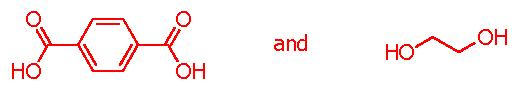
\includegraphics[width=0.5\textwidth]{\figpath/exercises-AABBesterification.pdf}}
		
				Here, we have taken the monomers shown in Step 1 of Model \ref{\labelbase:mdl:PET} and just replaced the methyl esters with carboxylic acids so that the reaction will be an esterification reaction rather than a trans-esterification reaction.
				}
				
			\end{solution}
			
			\item ... transesterification of an AB-type monomer:
			
			\begin{solution}
				\instructordisplay{
		
				A monomer that could be used to produce PET by transesterification of an AB-type monomer is
		
		\centerline{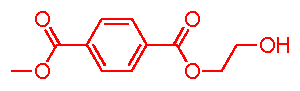
\includegraphics[width=0.3\textwidth]{\figpath/exercises-ABtransesterification.pdf}}
		
				Here, we have kept the methyl ester on the left-hand side, and linked on a single ethylene glycol unit to put a hydroxyl on the right-hand side.		
				}
			\end{solution}
			
			\item Both the AA+BB-type trans-esterification shown in Model \ref{\labelbase:mdl:PET} and the AA+BB-type esterification you drew in part (a) of this problem are used commercially to produce PET.  However, PET is never (or only rarely) produced from AB-type monomers.  Why do you think this is true?
			
				\begin{solution}
				\instructordisplay{
					The AB-type monomer shown in the solution to part (b) of this question is difficult to prepare in high purity, because the reagents have different reactive functional groups on both ends.  Preparing this monomer requires extra purification steps, which are generally too costly to make them industrially viable.
					}
				\end{solution}
			
			\end{enumerate}
		
		\exercise Although our focus in this exercise was on how to increase the degree of polymerization by removing the small-molecule byproduct, it is sometimes advantageous to push the equilibrium in the other direction.
		
			If you were to take a sample of PET and heat it in the presence of a large excess of water, what products would you expect to result?  Propose at least one application in which this process might be useful.
		
			\begin{solution}
				\instructordisplay{
				If PET is heated in the presence of water, we would expect the ester bonds to hydrolyze, forming terepthalic acid and ethylene glycol:
		
		\centerline{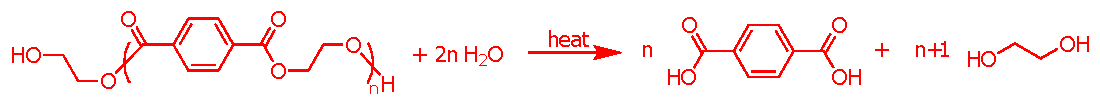
\includegraphics[width=\textwidth]{\figpath/exercises-PEThydrolysis.pdf}}
				
				When \emph{making} PET and using it to form new products, manufacturers typically try to avoid this reaction by thoroughly drying the polymer before molding it (which requires elevated temperatures). At the end of the life of a PET-based product, however, this sort of depolymerization can be used to recycle the plastic by recovering the starting materials.
				
				Note: most PET is not actually recycled by depolymerization - the polymer is instead cleaned, shredded, and re-molded into new products.  This process is typically more cost-competitive than chemical recycling.  However, similar hydrolysis reactions are used for other polyesters, and are also important for applications like controlled drug delivery (where slow degradation of a polyester in the presence of water facilitates slow release of a pharmaceutical compound - see e.g. \url{https://www.ncbi.nlm.nih.gov/pmc/articles/PMC3347861/}.)
				}
			\end{solution}
			
		%\exercise The polymerization of PET is an example of a \emph{transesterification} reaction.
		%	In Model \ref{\labelbase:mdl:PET}, we used transesterification of small molecule monomers to form a polymer.
		%	However, transesterification reactions can also take place between polymer chains, as well.
			
		%	What product would you expect to result from transesterification of the following two polymers?
		
		%	% Would be excellent to relate this to a result from the literature!
		
\end{exercises}
	
\end{activity}